\documentclass{beamer}
\usepackage[utf8]{inputenc}
\usepackage[english, ngerman]{babel}
\usepackage{tikz}
\usepackage{graphicx}
\usepackage{svg}
\usepackage{amsmath}
\usepackage{mathtools}
\usepackage{subcaption}
\usepackage{listings} 
\usepackage{color}

\definecolor{mygreen}{rgb}{0,0.6,0}
\definecolor{mygray}{rgb}{0.5,0.5,0.5}
\definecolor{mymauve}{rgb}{0.58,0,0.82}

\lstset{ 
  backgroundcolor=\color{white},   % choose the background color; you must add \usepackage{color} or \usepackage{xcolor}; should come as last argument
  basicstyle=\footnotesize,        % the size of the fonts that are used for the code
  breakatwhitespace=false,         % sets if automatic breaks should only happen at whitespace
  breaklines=true,                 % sets automatic line breaking
  captionpos=b,                    % sets the caption-position to bottom
  commentstyle=\color{mygreen},    % comment style
  deletekeywords={...},            % if you want to delete keywords from the given language
  escapeinside={\%*}{*)},          % if you want to add LaTeX within your code
  extendedchars=true,              % lets you use non-ASCII characters; for 8-bits encodings only, does not work with UTF-8
  frame=single,	                   % adds a frame around the code
  keepspaces=true,                 % keeps spaces in text, useful for keeping indentation of code (possibly needs columns=flexible)
  keywordstyle=\color{blue},       % keyword style
  language=Python,
  morekeywords={*,...},            % if you want to add more keywords to the set
  numbers=left,                    % where to put the line-numbers; possible values are (none, left, right)
  numbersep=5pt,                   % how far the line-numbers are from the code
  numberstyle=\tiny\color{mygray}, % the style that is used for the line-numbers
  rulecolor=\color{black},         % if not set, the frame-color may be changed on line-breaks within not-black text (e.g. comments (green here))
  showspaces=false,                % show spaces everywhere adding particular underscores; it overrides 'showstringspaces'
  showstringspaces=false,          % underline spaces within strings only
  showtabs=false,                  % show tabs within strings adding particular underscores
  stepnumber=2,                    % the step between two line-numbers. If it's 1, each line will be numbered
  stringstyle=\color{mymauve},     % string literal style
  tabsize=2,	                   % sets default tabsize to 2 spaces
  title=\lstname                   % show the filename of files included with \lstinputlisting; also try caption instead of title
}

\title{Elasticsearch presentation}
\author{University Stuttgart | IMS \newline Course: Texttechnology \newline Superviser: Andre Blessing \newline Students: Brandon Sorensen, Haywood Shannon, \newline Johannes Krämer, King DeLaney\newline WS 2018/19}

\date{}
\setbeamertemplate{navigation symbols}{}
\usetheme{PaloAlto}

%personalized colortheme
\setbeamercolor{frametitle}{bg=cyan!15!white, fg=cyan!70!green!60!white} 
\setbeamercolor{sidebar}{bg=cyan!70!green!60!white} 
\setbeamercolor{logo}{bg=cyan!35!white}
\setbeamercolor*{title}{bg=cyan!15!white, fg=cyan!70!green!60!white}

\lstset{language=Python}  
%i took this peace of code from 
%http://tex.stackexchange.com/questions/89885/remove-title-and-name-from-sidebar-yet-keep-them-in-the-bottom-part-of-the-prese
%in order to supress the long author name (where i also included the metadata) in the sidebar
  \makeatletter
  \setbeamertemplate{sidebar \beamer@sidebarside}%{sidebar theme}
  {
    \beamer@tempdim=\beamer@sidebarwidth%
    \advance\beamer@tempdim by -6pt%
    \insertverticalnavigation{\beamer@sidebarwidth}%
    \vfill
    \ifx\beamer@sidebarside\beamer@lefttext%
    \else%
      \usebeamercolor{normal text}%
      \llap{\usebeamertemplate***{navigation symbols}\hskip0.1cm}%
      \vskip2pt%
    \fi%
  }%
\makeatother

%i used a sidebar instead of ToC
\begin{document}
\begin{frame}
\maketitle
\end{frame}

\section{Elasticsearch}
\begin{frame}
\frametitle{Elasticsearch}
\begin{itemize}
\item it's a database
\pause
\item it's also a search engine (optimized for text)
\pause
\begin{itemize}
\item boolean search
\item phrase search / proximity search
\item wildcard queries
\item term weighting
\item aggregation
\end{itemize}
\pause
\item implemented in java, on top of lucene
\item incredibly fast
\item RESTful (libraries are available e.g. for Python)
\item no-sql $\rightarrow$ schema-less $\rightarrow$ example
\end{itemize}
\end{frame}

\section{Schema-less example}
\begin{frame}
\frametitle{The Pokemon Example}
\begin{figure}
\centering  
\begin{subfigure}{.8\textwidth}
    \centering  
    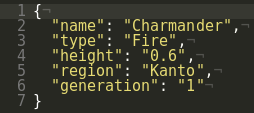
\includegraphics[width=0.8\textwidth]{Pokemon1.png}
  \caption{Charmander pokedex entry}
\end{subfigure}%
\pause
\begin{subfigure}{.2\textwidth}
  \centering  
  
\includegraphics[width=0.5\textwidth]{Charmander.png}
\end{subfigure}
\end{figure}
\end{frame}

\begin{frame}
  \frametitle{The Pokemon Example}
  \begin{figure}
  \centering  
  \begin{subfigure}{.8\textwidth}
      \centering  
      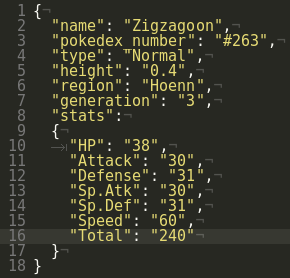
\includegraphics[width=0.8\textwidth]{Pokemon2.png}
    \caption{Zigzagoon pokedex entry}
  \end{subfigure}%
  \pause
  \begin{subfigure}{.2\textwidth}
    \centering  
    
\includegraphics[width=0.8\textwidth]{Zigzagoon.png}
  \end{subfigure}
  \end{figure}
\end{frame}

\section{The real power}
\begin{frame}
  \frametitle{ELK Stack}
    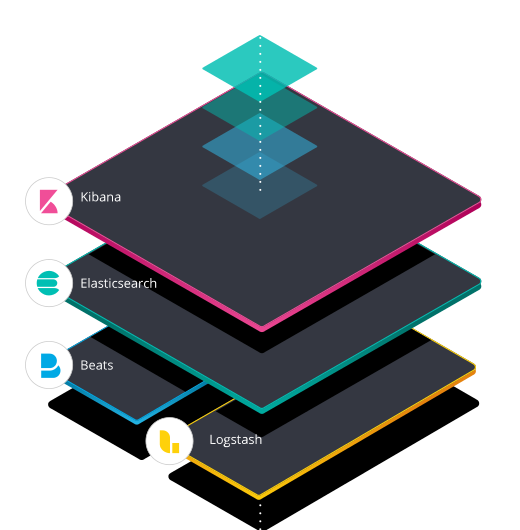
\includegraphics[width=0.8\textwidth]{ELK.png}
\end{frame}

\section{Logstash}
\begin{frame}
  \frametitle{Logstash Python vs. Conf}
  \begin{enumerate}
   \item Logstash is a preprocessing tool 
  \end{enumerate}
  \lstinputlisting[language=Python, firstline=30, lastline=40]{indexit.py}
\end{frame}
\begin{frame}
  \frametitle{Logstash Python vs. Conf}
  \lstinputlisting[language=Python, firstline=2, lastline=7]{ufoindex.conf}
\end{frame}
\begin{frame}
  \frametitle{Logstash Python vs. Conf}
  \lstinputlisting[language=Python, firstline=8, lastline=22]{ufoindex.conf}
\end{frame}
\begin{frame}
  \frametitle{Logstash Python vs. Conf}
  \lstinputlisting[language=Python, firstline=23, lastline=34]{ufoindex.conf}
\end{frame}

\section{Kibana}
\begin{frame}
  \frametitle{Kibana}
  Kibana demo
\end{frame}

\section{Conclusion}
\begin{frame}
  \frametitle{Conclusion}
  \begin{enumerate}
   \item don't confuse it with a NLP tool, it's not
   \item not recommended for PROD $\rightarrow$ not stable
   \item fast changes (e.g. deprecations) with releases $\rightarrow$ careful with old tutorials
   \item remarkable $\rightarrow$ get insights into data in no time
  \end{enumerate}
\end{frame}


\end{document}